%%%%%%%%%%%%%%%%%%%%%%%%%%%%%%%%%%%%%%%%%%%%%%%%%%%%%%%%%%%%%%%%%  
% For submission to AUTOMATICA as a communique for fast publication.
% Draft by Dr YangQuan Chen @11.01.0.  
% Motivated by Prof. Kevin L Moore of CSOIS/ECE/USU
%%%%%%%%%%%%%%%%%%%%%%%%%%%%%%%%%%%%%%%%%%%%%%%%%%%%%%%%%%%%%%%%%  

 
%\documentclass[a4,technote,12pt,twoside]{ieeetran}
%\documentclass[a4,12pt,twoside]{ieeetran}
\documentclass{cdcarta4}
%\documentclass[a4,10pt,twoside,twocolumn]{ieeetran}
%\documentclass[a4,12pt]{ieeetran}
%\usepackage[dvips]{epsfig} 
%\usepackage{subfigur} 
\usepackage{alltt,graphicx,hyperref}
%\bibliographystyle{c:/pctexv4/texinput/ieeebib}
\bibliographystyle{ieeebib}
\renewcommand{\baselinestretch}{0.92}


\begin{document}
  

\title{{\vspace*{-1cm} \hspace*{12.5cm} \Large \bf IEEE ISIC'02}
\\
 \Large \bf  
Some Sensing and Perception Techniques for  an Omnidirectional Ground Vehicle
With a Laser Scanner
\thanks{Jan. 2002.  {\em For submission to IEEE International Symposium on Intelligent Control (ISIC'02)},  Oct. 2002, Vancouver, Canada, as an invited session paper.   Invited Session   organized by Dr  Jason Gu.
This work is supported in part by U.S. Army Automotive and Armaments Command (TACOM)
 Intelligent Mobility Program (agreement no. DAAE07-95-3-0023. Corresponding author: Dr YangQuan Chen. E-mail:  \texttt{yqchen@ieee.org}; Tel. 01-435-7970148; Fax: 01-435-7972003. URL: \texttt{http://www.crosswinds.net/\char126 yqchen}. 
} 
}


\author{
Zhen Song,   YangQuan Chen,  Lili Ma and   You Chung Chung\\ \\
 Center for Self-Organizing and Intelligent Systems (CSOIS),  \\
Dept. of Electrical and Computer Engineering,  4160 Old Main Hill, \\
Utah State University, Logan, UT 84322-4160, USA. \\
}
     
    
\maketitle

\begin{abstract}                          % Not more than 200 words.
This paper presents some techniques for sensing and perception for an
omnidirectional ground autonomous vehicle equipped with a laser scanner. In an
assumed structured environment, the sensing data processing methods for both 1D
and 2D laser scanner are discussed. Raw data are segmented to lines, circles,
ellipse, planes and corners by task depended segmentation algorithms.  Each
subset of data is then fit by a known template shape as listed above.  With
these medium level information, the vehicle can infer its relative position with
respect to the known landmarks and in turn help to determine its absolute
position on the map.
%\begin{keyword}   % Five to ten keywords,  
\\
{\bf Key Words: } 
 Hough transform;
 line fitting;
 corner fitting;
 arc/circle fitting;
 ellipse fitting;
 algebraic fitting;
 %geometrical fitting;
 weighted circle fitting;
 Omni-directional vehicle (ODV).
%\end{keyword}                             % keyword list.
\end{abstract}

% sorry, I have to use the following preambles
% apologize for any inconvenience caused!

\newtheorem{remark}{Remark}[section]
%%% defines the QED square and the proof environment
%\def\QED{~\rule[-1pt]{5pt}{5pt}\par\medskip}
%\newenvironment{proof}{{\bf Proof: \ }}{ \hfill \QED}
\def\etal{ {\em et  al. }}
\def\K{ $^\circ{\rm K}$ }
\def\norml{\parallel\!\!}
\def\normr{\!\!\parallel}
\def\eqdef{\stackrel{\triangle}{=}}
\def\rd{\partial}
\def\ba{\begin{array}}
\def\ea{\end{array}}                                    
\def\be{\begin{equation}}
\def\ee{\end{equation}}
\def\bi{\begin{itemize}}
\def\ei{\end{itemize}}
\def\bea{\begin{eqnarray}}
\def\eea{\end{eqnarray}}
\def\btb{\begin{tabular}}
\def\etb{\end{tabular}}
\def\ne{ \nonumber \\ \, }
\def\ca{\citeauthor}
\def\d{ {\rm  d} }
\newtheorem{thm}{Theorem}[section]
%\newtheorem{remark}{Remark}[section]

%%%%%%%%%%%%%%%%%%%%%%%%%%%%%%%%%%%%%%%%%%%%%%%%%%%%%%%%%%%%%%%%%%%%%%%%%%%%
\section{Introduction}
\label{sec1}
%%%%%%%%%%%%%%%%%%%%%%%%%%%%%%%%%%%%%%%%%%%%%%%%%%%%%%%%%%%%%%%%%%%%%%%%%%%%   
 

%{\em To be finished by Dr Chen.}

\subsection{Motivation}

For any intelligent mobile robot, the perception of its environment via suitable sensing capacities plays a key role \cite{Adams99,Nourbakhsh97}. The  environment perception depends largely on the properties of environment itself. Basically, the environment can be assumed to be either static (deterministic) such as office corridor  or dynamic (changing) such as a   parking lot with vehicles in and out dynamically. In terms of 
deterministicism of the environment, there are two types: deterministic environment and uncertain environment.
With combination, we have four types of environments: static deterministic, dynamic deterministic, static uncertain and dynamic uncertain. For static and dynamic deterministic environments, the sensing and perception task is easier with a help of a map and the known motion patterns of the objects in the environment. For uncertain environment, it seems no {\em off-the-shelf} solution exists for general sensing and perception tasks for mobile robots \cite{Adams99}. This is because,  sensing and perception  solutions  are usually {\em platform-specific}  for mobile robot with given or existing sensing capability \cite{Adams99,Nourbakhsh97}. However, there are still some common and possibly low-level solutions applicable for all platforms. This paper attempts to present some commonly used  techniques for sensing and perception for  mobile robot equipped with a 1D or 2D laser scanner in static uncertain environment.
%
Our test platform is an omni-directional ground autonomous vehicle developed in the CSOIS at Utah State University (USU).



Our approach for static uncertain environment perception is based on the following steps (1) laser scan raw data, (2) segmentation, (3) fitting from the object library (or template objects), (4) object arbitration or decision. 
For step-1, pre-processing is performed to reject some obviously abnormal points or outliers.
In step-2, the range data array from a laser scan is to be segmented to form some subsets of point clouds containing essential information for the object fitting. We assume that a library of objects such as line, corner/rectangle, arc/circle/ellipse etc. are available from the prior knowledge about the static uncertain environment.
Then in step-3, we fit the through the library since we do not know in advance which object the given point cloud represents. The arbitration or decision on which object in step-4 is done by a rule based comparison of the fitting scores. We believe that this procedure is natural and can be regarded as a common piece of utility in sensing perception using a laser scanner. In each step of the above proposed procedure, there are many technical as well as theoretical challenges. In the present paper, we shall more focused on step-3. 

The major contribution of this paper is the collection of some commonly used object fitting algorithms well tested in our experiments with our C++ and Matlab codes publically available 
\footnote{In the final version of this paper, we will give an URL for downloading the object fitting codes developed in this paper.}.


\subsection{The USU ODIS/T4 Platform}

The USU ODIS  robot is   a small, man-portable mobile robotic system that can be used for autonomous or 
 semi-autonomous inspection under vehicles in a parking area \cite{moore_csm}. Customers for such a system include military police (MP) and other law enforcement and security entities. The robot features (a) three ``smart wheels''  in which both the speed and direction of the wheel can be independently controlled, (b) a vehicle electronic capability that includes multiple processors, and (c) a sensor array with a laser, sonar and IR sensors, and a video camera. ODIS employs a novel parameterized command language for intelligent behavior generation. A key feature of the ODIS control system is the use of an object recognition system that fits models to sensor data. These models are then used as input parameters to the motion and behavior control commands.
Fig.~\ref{fig:odis1} shows the mechanical layout of the ODIS robot. The robot is 9.8 cm tall and weighs approximately 20 kgs. Key ODIS subsystems include its mechanical, vehicle electronics (vetronics) and sensor systems.  For more detailed description, see ~\cite{odis_spie01}~\cite{odis_icra01}.
%
%
\begin{figure}[!htb]
%\centerline{\epsfig{file=odis1.eps,width=7.cm,height=4.5cm}}
    \center
    \includegraphics[width=7.cm,height=4.5cm]{img/odis1}
    \caption{The mechanical and vetronics layout of ODIS}  \label{fig:odis1}
\end{figure} 


Fig.~\ref{odis1blk} shows the behavior control architecture that has been developed. 
Starting from the "inside out," the control architecture contains two inner motion-control loops. The inner most loop is the wheel-level control, which acts to drive each smart wheel to its desired steering and drive speed set-points. The wheel-level controller uses simple PID control algorithms. Around the inner loop is the path-tracking controller. This loop derives the set points need by the wheel-level control in order to force the vehicle to follow a desired path in space, where a path is defined as an arc in inertial space (with a prescribed velocity along the arc) and an  associated vehicle yaw motion. The path-tracking controller 
uses a newly-developed spatial tracking control algorithm that is described in more detail in  \cite{odis_icra01}. 

\begin{figure}[!htb]
%\centerline{\epsfig{file=odis1blk.eps,width=8.3cm}}
\center
\includegraphics[width=8.3cm]{img/odis1blk}
%\vspace*{6cm}
\caption{The behavior control system architecture of ODIS} 
\label{odis1blk}
\end{figure} 

Fig.~\ref{fig:1dlaser} shows the 1D laser scan data for a typical set of objects in front of the ODIS equipped with a 1D laser. In our project, objects in parking lots can be  decomposed into  combinations of  arcs/circles and lines/rectangles. 
\begin{figure}[!htb]
    \center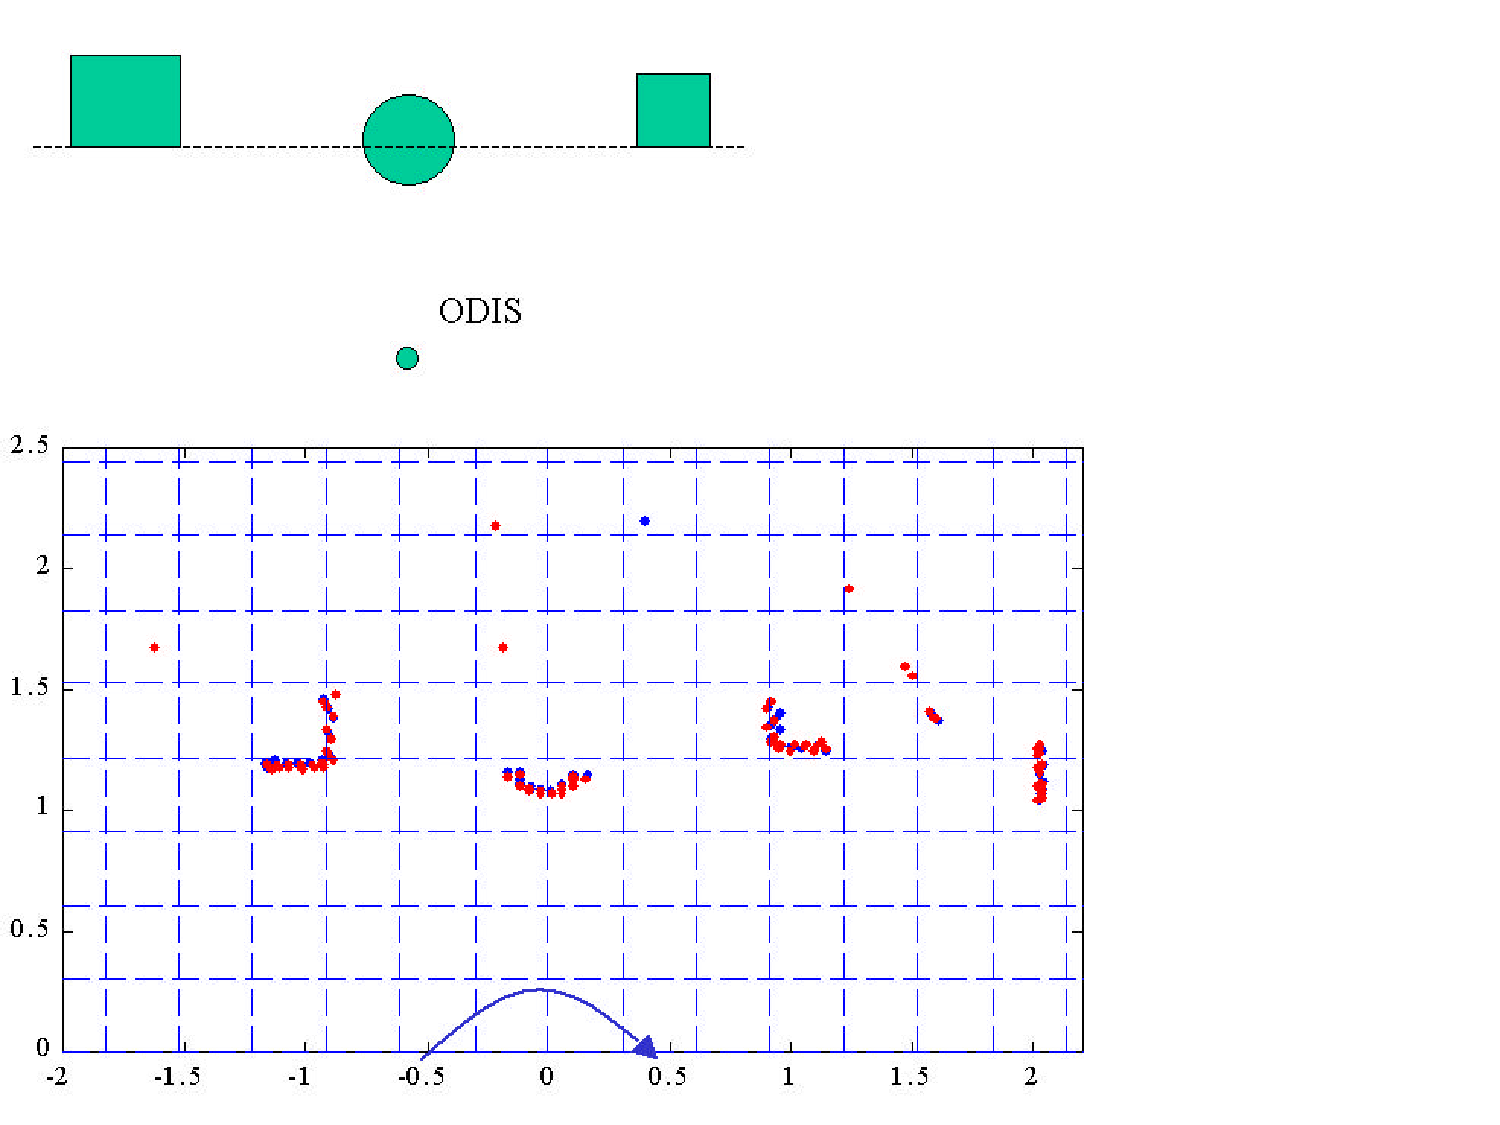
\includegraphics[width=0.4\textwidth]{img/1Dlaser}
    \caption{1D Laser Data (Top: Object Setting.  Bottom: Laser Data)}
\label{fig:1dlaser}
\end{figure}


Currently, the cost of a 2D laser scanner is greatly, which enables increasingly many robots be equipped with 2D laser scanner. Again, ``{\em off-the-shelf}'' algorithms for object identification  or for environment features extraction have not been available although some very platform-specific schemes are proposed or tried, e.g., the research work reported in \cite{Dedieu00Mixed,Hartmart2001ISR,Taylor1996,Vandorpe1996,Cadenat2000,Laurent1997,Borenstein96WhereAmI}.
Fig.~\ref{fig:2dlaser} shows the coordination system of our 2D SICK laser \footnote{\texttt{http://www.sickoptic.com/kommerce\_server/}}. For computational  convenience, it is different from the body frame coordination system (BFCS) and inertial coordination system (ICS). The height of 2D laser above ground, denoted by $h$,  is  constant. From the data of 2D laser scanner, we can get a set of raw data points $(x',y')$ together with  the corresponding pitch angle $\alpha$ from the tilting servo system. To convert  the raw data  into 3D coordination system $(x,y,z)$, we have
$   \beta={\rm atan} (y'/x')  $ and $ d = \sqrt{x'^2 + y'^2} $. So, we get $ (x,y,z)=(d \cos(\beta)\sin(\alpha), d \sin(\beta), h-d \cos(\alpha)\cos(\beta) )$.
In Sec.~\ref{sec3}, we will introduce some object fitting algorithms such as plane fitting (Sec.~\ref{sec3_planefit}), 3D corner detection  and  fitting (Sec.~\ref{sec3_3dcornerfit}), and etc. for 2D laser scanner.

\begin{figure}[!htb]
    \center\includegraphics[width=0.45\textwidth]{img/2Dlaser}
    \caption{2D Laser Coordinate System }
\label{fig:2dlaser}
\end{figure}



The rest of the paper is organized as follows. 
Sec.~\ref{sec2} presents a revised Hough transform method
for an efficient segmentation of the laser scan raw data set.
Also in this section, lamp pole simulation data are presented to give
an example of task depended segmentation.
A set of fitting algorithms are described in Sec.~\ref{sec3} which includes both 1D  and 2D laser data processing such as line or plane fitting, circle fitting, 3D corner fitting etc. 
%
Finally, Sec.~\ref{sec6} concludes this paper with some remarks on our on-going research efforts.


 

%***************************************************
\section{Segmentation}
\label{sec2}


\subsection{Line Detection for Segmentation}
\label{sec21}


Line detection is the first step to segment 1D laser data. After the line detection, we can judge if a point is on the line by checking the distance between the point and the line. In our project, it is reasonable to segment objects in parking lots to circles and lines. So segmentation is simplified as line detection and circle fit. 

There are many paper published on line detection. Some took the frequency-domain approach ~\cite{HuaLineFitting} and others took time-domain approach, e.g. Hough Transform ~\cite{HoughSurvey}, or color pattern analyze~\cite{Jan00model}. In our project, the input is sequential laser data, instead of image. In the following discussion, we will focus on Hough Transform.

%
Hough Transform (HT) is a popular method for the extraction of geometric primitives \cite{HoughSurvey,Atherton99CHT}. At the beginning, it is only an approach for line detection. Later, many variant are developed, thus this algorithm can detect circle~\cite{Atherton99CHT}, ellipse~\cite{guil97lower}, or more complex binary patterns~\cite{guil96new}. The survey on Hough Transform~\cite{HoughSurvey} gives a good big-picture on the current research progress. 

Generally speaking, HT is robust to sensor noise at the expense of slow computation. The compensational cost  of the traditional HT is   $O(n^3)$ where $n$ is the number of data points. Though some efforts were made to speed up the HT algorithm~\cite{matas98progressive}, those fast strategies were developed generally for  image data processing applications only. 


However, in our case,  1D laser data set
contains only {\em sparse}  
  binary information in the region of interest. Furthermore,  only 1D array is requred for laser data instead of 2D  matrix for image data. More importantly, 
 the laser data set is  sequential or ordered. Taking these properties of laser data set, HT can be modified to reduce the computational time. 



\subsection{Sparse Hough Transform for 1D Line Detection}
\label{sec22}

In order to make the most use of those valuable features of laser scanner data set, 
 here we propose a Sparse Hough Transform (SPHT) that fit better to the laser data processing problem. The Standard Hough Transform (SHT) represents lines crossing a point by 
%
$$ \rho = x \cos\theta + y \sin\theta, $$
%
where $\rho$ and $\theta$ are the length of the normal and the angle of the normal with respect to the positive $x$-axis. $x$ and $y$ are the coordinates of a   point of interest in the image.   $\rho$ and $\theta$ are quantified as the dimensions of an accumulator matrix. The value of each cell of the matrix represents how many times there is a line, denoted by $(\rho, \theta)$, passed a point in the image. The idea of Sparse Hough Transform is to provide an equivalent but faster and less memory-demanding approach. Basically, SPHT does not use a 2D array to record the votes. Instead, it uses a 1D  array to do the same vote-counting job. Since in sparse case, most lines passed one point are not the fitted lines, we can compute only those lines that passed at least two points in the image. Transfer all the lines corresponding to one point in the image plant, as SHT does, would take extra computer memory and reduce the speed. 


Based on the above considerations, we present an 
 implementation of SPHT by the following   pseudo-code list:\\
(\texttt{Dat} is the input array; \texttt{Dat(n).x} is the $x$ value of the $n$-th point. 
\texttt{Lines} is the output array that stores $(\rho,\theta)$ of the fitted lines.
\texttt{NumLen}=0, which is the number of fitted lines.)

{\footnotesize
\texttt{for i=1 to n-1}\\
\hspace*{4mm}    \texttt{for j=i+1 to n} \\
\hspace*{8mm}                $\alpha$ = atan($\frac{ Dat(i).y- Dat(j).y}{Dat(i).x - Dat(j).x} $)\\
\hspace*{8mm}                $\rho_0$ = (Dat(i).x cos($\alpha$ -$\pi$/2) + Dat(j).y sin($\alpha-pi/2$)\\
\hspace*{8mm}                $\theta$= $\alpha$-sign($\rho_0$) $\pi/2$ \\
\hspace*{8mm}                $\rho=|\rho_0|$ \\
\hspace*{8mm}                Cell$\theta$=floor($\theta$/$\Delta\theta$)*$\Delta\theta$ \\
\hspace*{8mm}                Cell$\rho$=floor($\rho/\Delta\rho$)*$\Delta\rho$ \\
\hspace*{8mm}                If line n, where $n\in[1,$NumLen]  is close enough to (Cell$\rho$,Cell$\theta$) increase the vote of Lines(n) by one, otherwise NumLen=NumLen+1 and add a line (Cell$\rho$, Cell$\theta$) to Lines with vote equates to one.  \\
\hspace*{4mm}    \texttt{end for} \\
\texttt{end for}
}
    
Fig.~\ref{fig:spht} shows an example of the proposed SPHT. The SPHT transforms or fits  the raw set data to 2 lines. 
Actually,  the raw data could be interpreted as 2 lines,  or 2 lines plus a small transit arc, or even just one line. The exact segmentation depends on the resolution, or the threshold. For example, with a  more precise laser sensor, we can know  that the data in Fig.~\ref{fig:spht} cannot be a single line. However, if  the data is from a low-precision sonar sensor, the target object might be just a single line. With a given sensor in real project, we could choose some reasonable thresholds by referring to the specifications of the sensors. Further discussions on the trade-off between sensor accuracy and the object fit accuracy can be found in~\cite{Goto98Efficient} and ~\cite{Goto00Design}.


\subsection{Analysis on Speed and Memory Size}
\label{sec23}

In general, suppose the  angle resolution is given by $\Delta\theta$ and normal resolution   $\Delta\rho$. For SHT,   $M\times N$ cells are required for the accumulation space, where $ M = \pi/\Delta\theta $ and  
$    N=\rho_{max}/\Delta\rho.  $
In other words, the   memory size is $n\times M\times N$, where $n$ is the size of each cell.
If there are $K$ valid points in the input data, the computation requirement is $O(K\times M)$.

For SPHT, if there are only $K$ valid points in the input, clearly $K\ll M$ and $ K \ll N$. The maximum number of fitted lines could be $ K\times (K-1)/2$. The computation requirement is then $O(K\times (K-1)/2) $. 

Figure~\ref{fig:sphtspeed} shows the computation cost of SPHT versus SHT when the image matrix/array has 100 by 100 points. In practice, in a  laser scan, the number of data point is  in the order of 10, i.e., the array  contains typically   only tens of valid data points.  From Fig.~\ref{fig:sphtspeed}, clearly, SPHT has a better performance  over SHT.


\begin{figure}
    \centering
    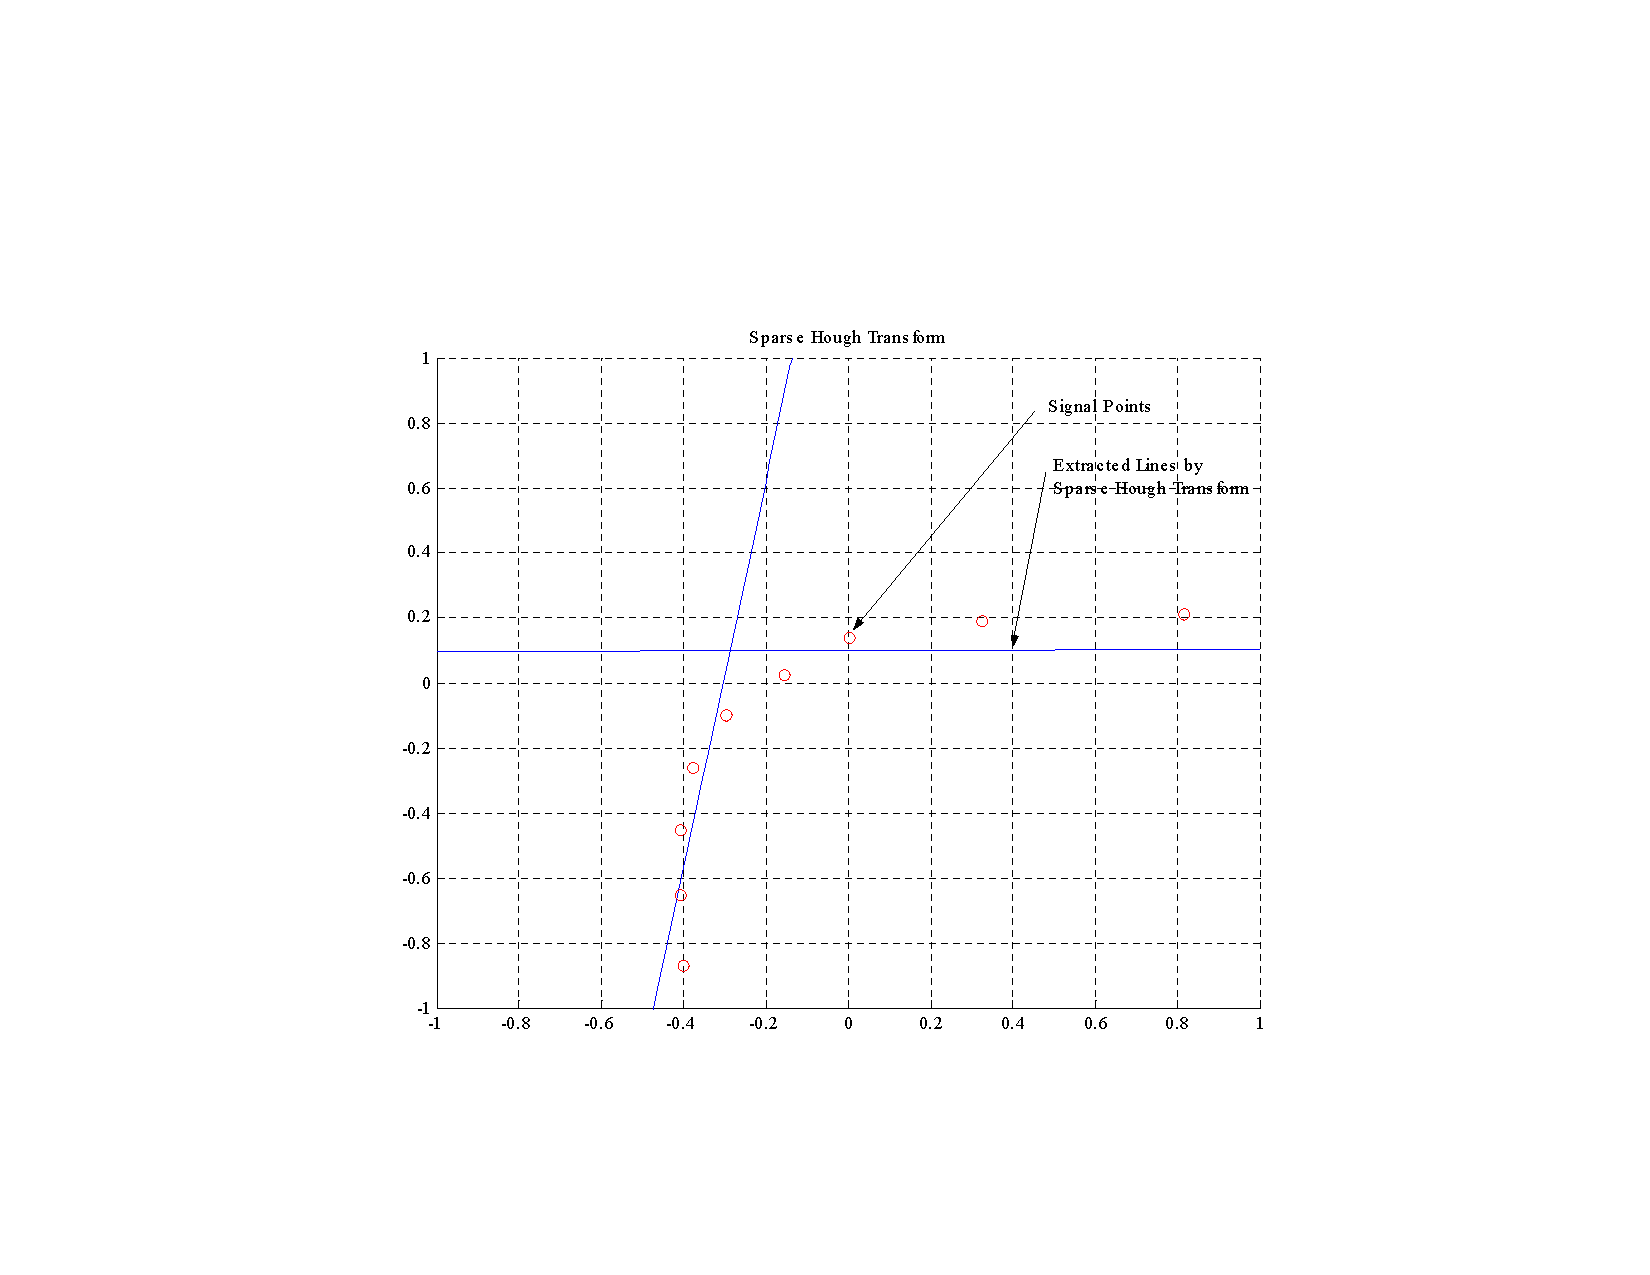
\includegraphics[angle=90,width=0.45\textwidth]{img/sparsehough}
    \caption{An Example of Sparse Hough Transform} \label{fig:spht}
\end{figure}

\begin{figure}
    \centering
    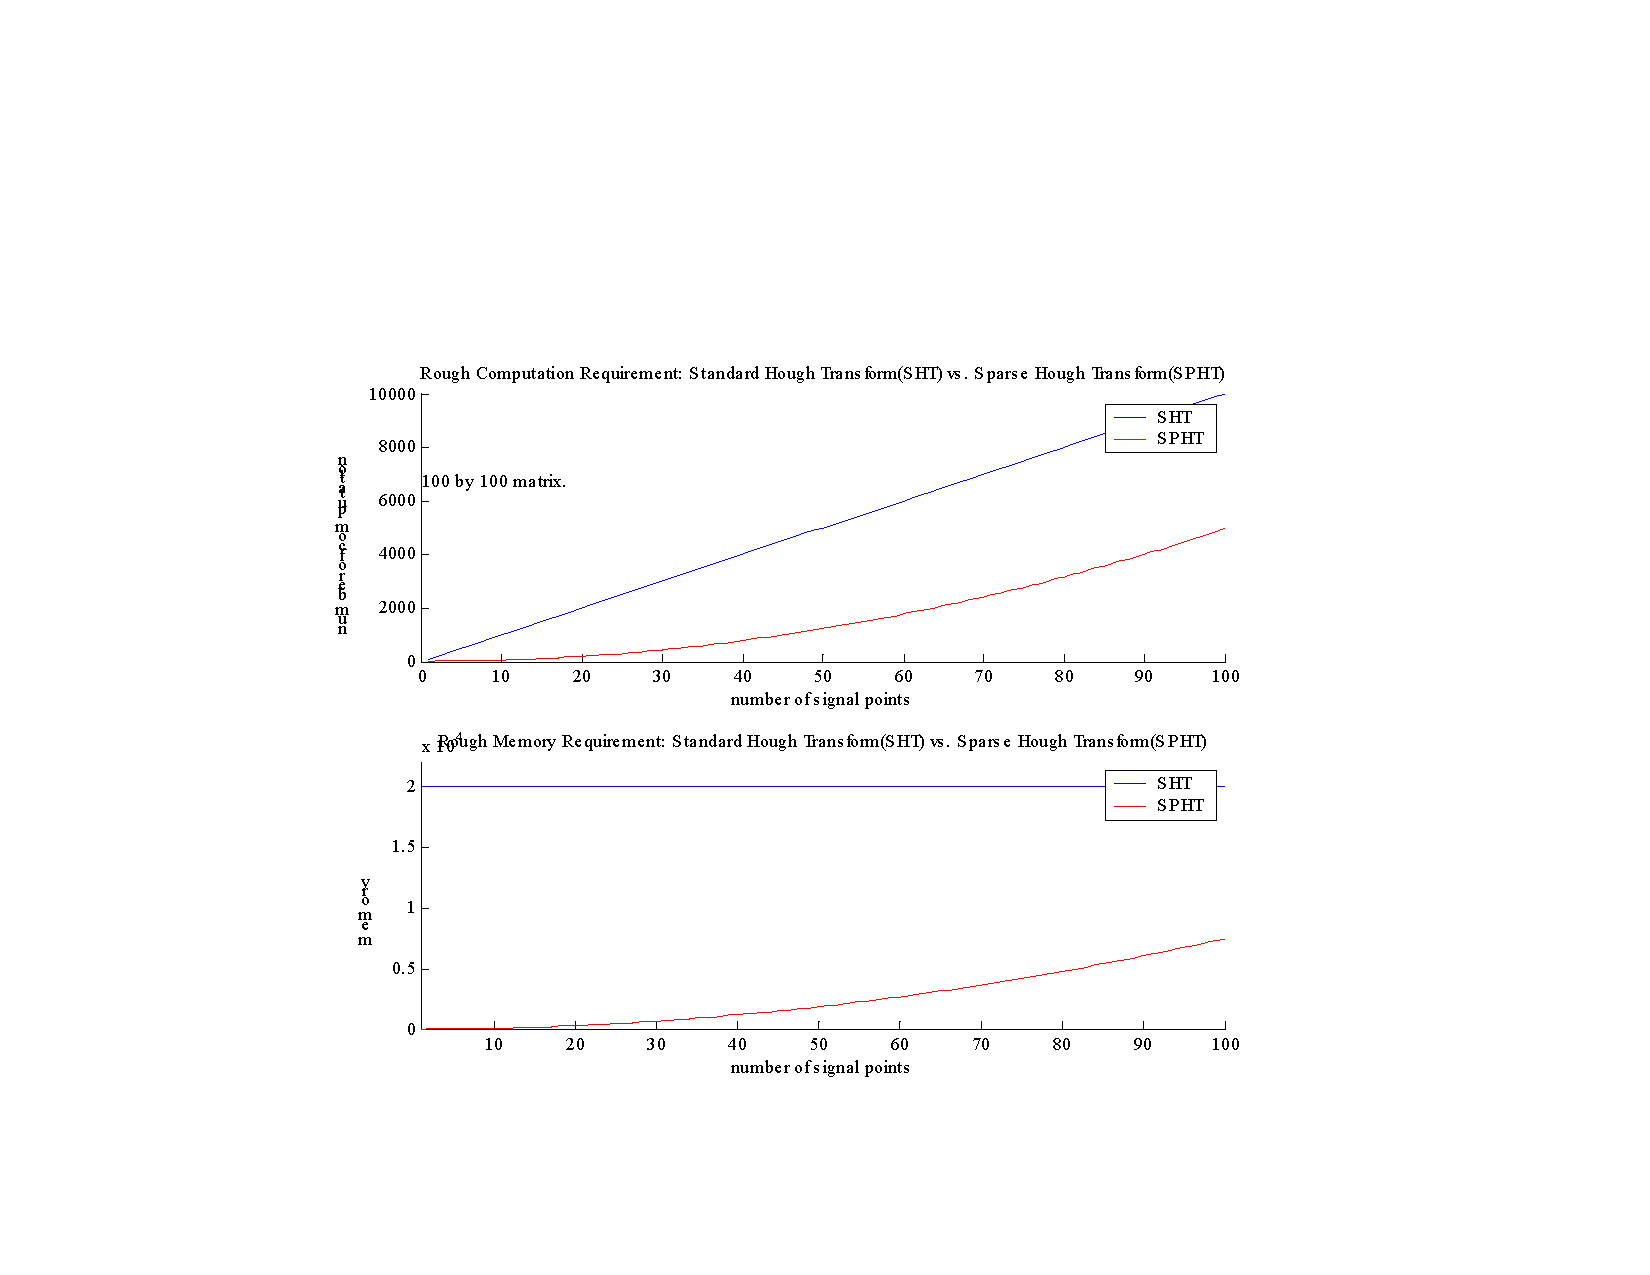
\includegraphics[angle=90,width=0.45\textwidth]{img/SSHTSpeed}
    \caption{Speed Comparison of SPHT and SHT} \label{fig:sphtspeed}
\end{figure}

%%%%%%%%%%%%%%%%%%pole fit
\subsection{Task-Dependent Segmentation}
\label{sec24}


To process 2D laser data, segmentation is more complicated than in the case of 1D laser data. The idea of task-dependent segmentation is to simplify the situation by make a better use of the known information. Currently, we use lamp pole and side walk as landmarks to calibrate the odometry system of the mobile robot.

Lamp pole is an important landmark in parking lot. Fig.~\ref{fig:polefit} is the simulated 
data of a lamp pole from a 2D laser scanner mounted on T4, the mother robot or vehicle for ODIS. Here we assumes the lamp pole is normal to the ground and ground is flat. The task is to segment the raw data so
that the position of the center of the lamp pole (cylinder) can be computed by some fitting algorithms. Some of these computations were done by Matlab functions. Fig.~\ref{fig:polefitimg} is the image that the lamp pole projected to the ground. Here we actually separate the ground from the lamp pole. Fig.~\ref{fig:polefitedge} is the result of edge detection of Fig.~\ref{fig:polefitimg}. Fig.~\ref{fig:polefitElm} is the 3D object when we re-project   the edge in Fig.~\ref{fig:polefitedge} back to 3D space. At last, we set a threshold to eliminate those points too close to each other, then we get Fig.~\ref{fig:polefitElm}. 

After projecting these points to the ground we get a circle with the same center of the 3D lamp pole. In other words, when we feed the result of the segmentation to our fitting algorithms, we can get the position of the feature points. Then the relative position of the landmark is available which can be used for mobile robot odometry calibration, or localization. 

Another important landmark is the convex corner of the side walk. Since the height of side walk in a specific parking lot is constant, we can set a threshold to segment the ground and upper layer. The segmentation is straightforward and  we will not discuss it here due to space limitation. 

\begin{figure}[!htb]
    \centering
    \begin{minipage}[t]{0.4\textwidth}
       \centering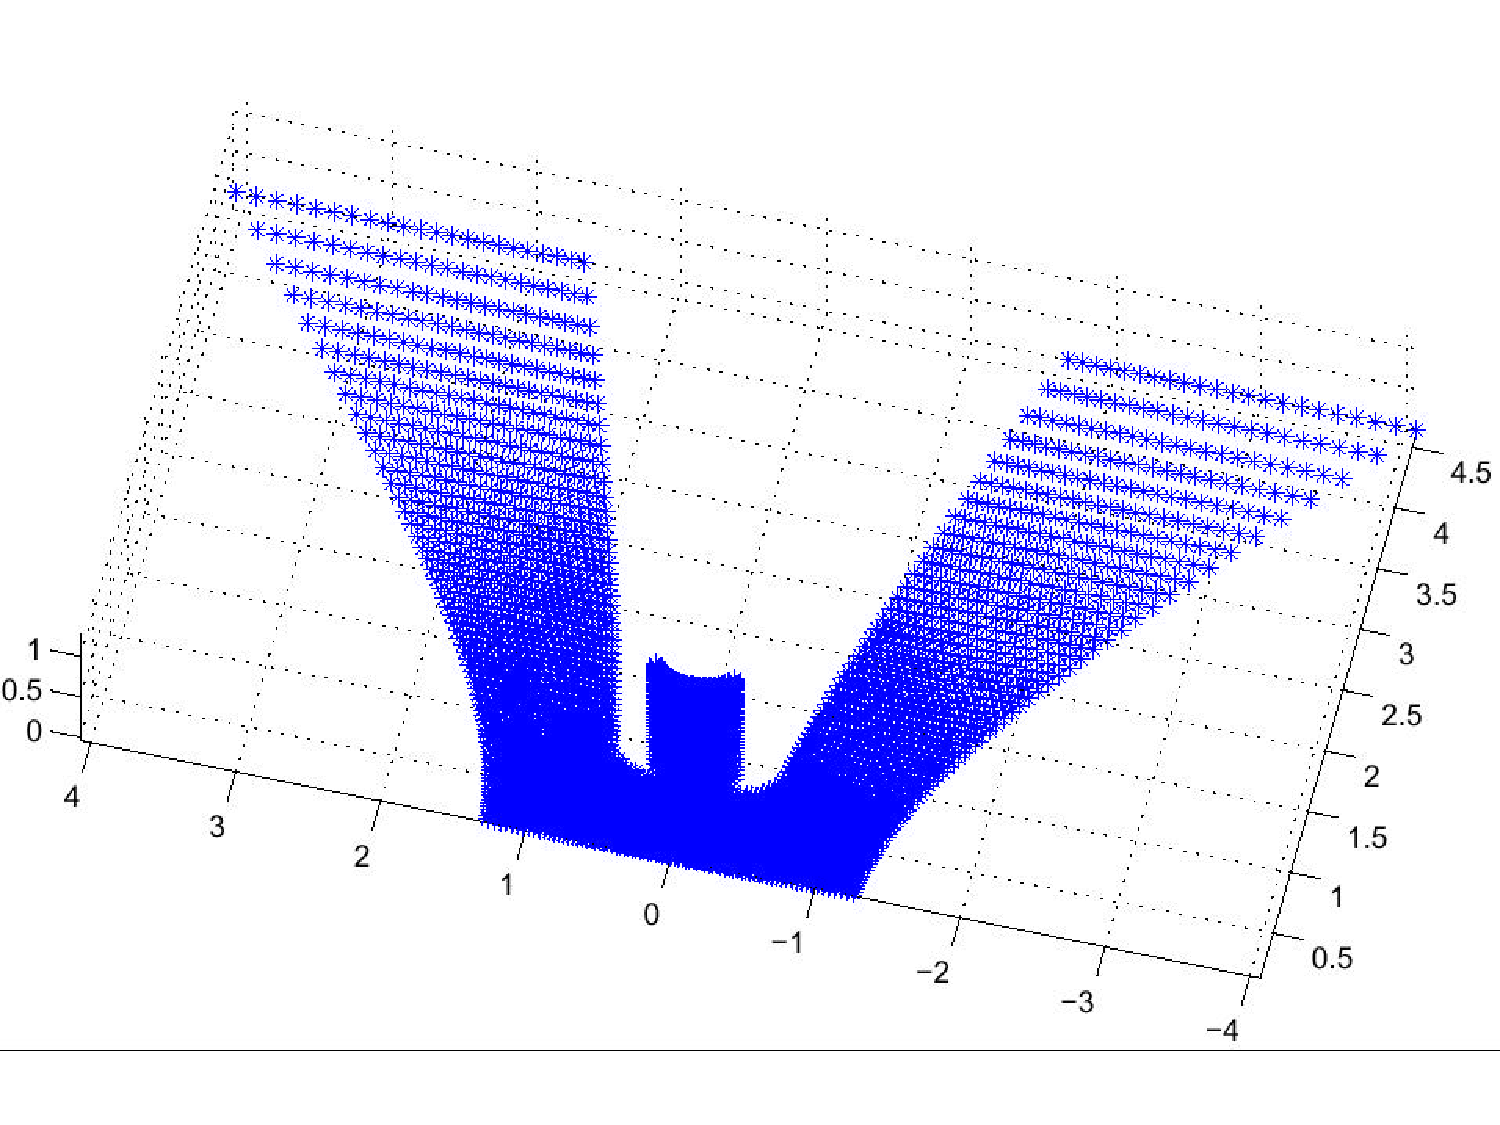
\includegraphics[width=\textwidth]{img/PoleFit}
       \caption{Lamp Pole Simulation Data} \label{fig:polefit}
    \end{minipage}
\end{figure}
\begin{figure}[!htb]
    \begin{minipage}[t]{0.23\textwidth}
       \centering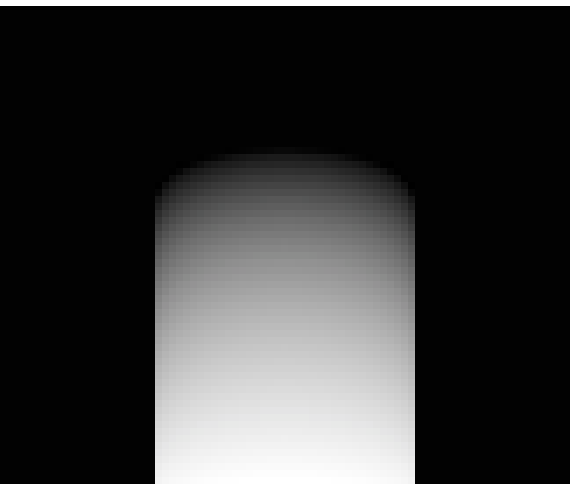
\includegraphics[width=\textwidth]{img/PoleFitImg}
       \caption{Projected Lamp Pole Image} \label{fig:polefitimg} 
    \end{minipage} %
    \begin{minipage}[t]{0.23\textwidth}
        \centering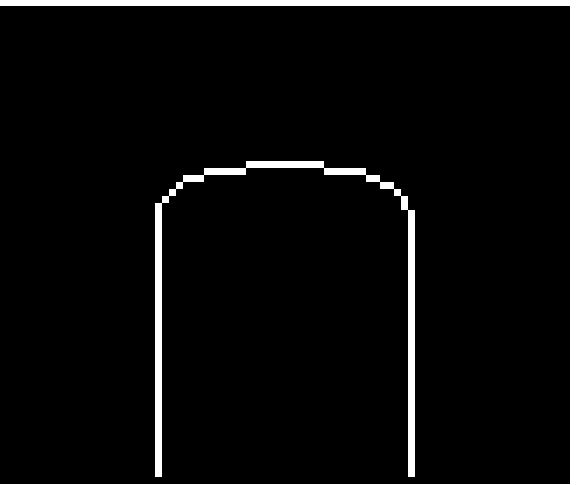
\includegraphics[width=\textwidth]{img/PoleFitEdge}
        \caption{The Edge Detection on Lamp Pole Image} \label{fig:polefitedge}
    \end{minipage}
\end{figure}
\begin{figure}[!htb]
    \begin{minipage}[t]{0.23\textwidth}
        \centering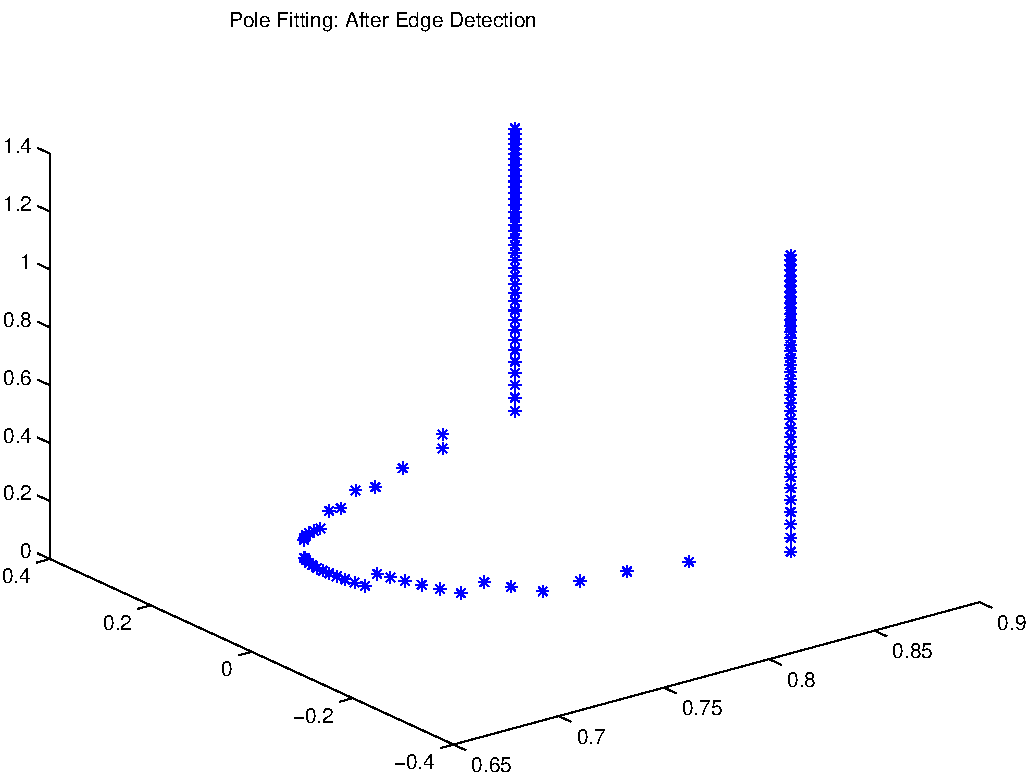
\includegraphics[width=\textwidth]{img/PoleFitAfterEdgeDet}
        \caption{Reverse The Edge of Lamp Pole Image} \label{fig:polefitafteredgedet}
    \end{minipage} %
    \begin{minipage}[t]{0.23\textwidth}
        \center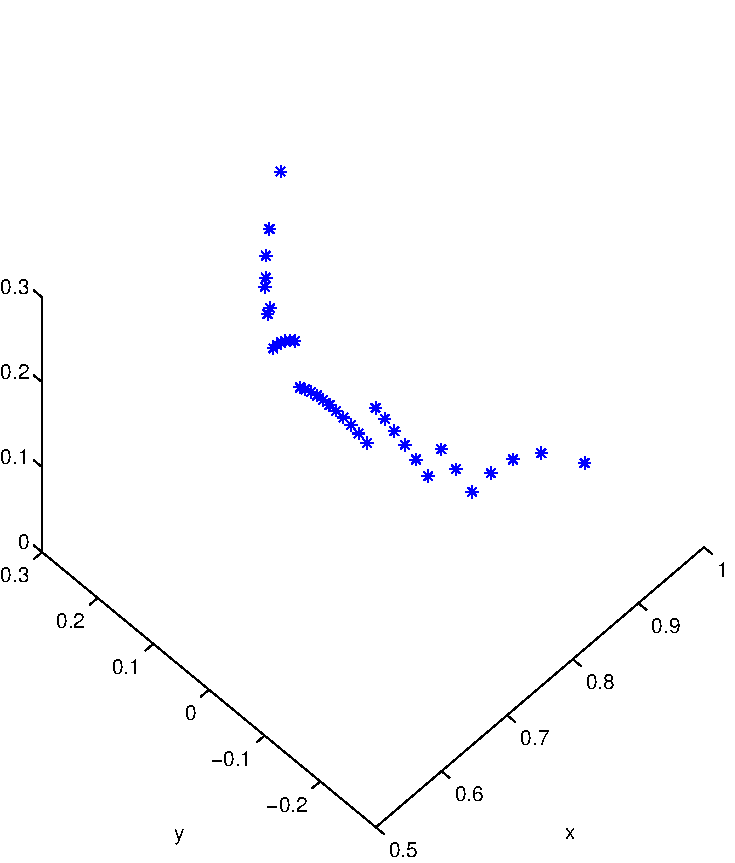
\includegraphics[width=\textwidth]{img/PoleFitEliminateStacks} 
        \caption{Lamp Pole Data After Segmentation} \label{fig:polefitElm}
    \end{minipage}
\end{figure}






%***************************************************
\section{Template Fitting Algorithms}
\label{sec3}

With  properly segmented data sets from a laser scan,  it is not certain which   template in the template library is to be used for the object fitting, without human involvement. A viable way is to try fit all templates in the library and then pick the ``best'' one via an arbitrator based on some rules from the possible prior knowledge about the objects in the static and uncertain environment.

For computational efficiency, we focus ourself on the algebraic fitting which does not require any iteration.
For geometrical fitting, is may make more sense but the iterations may take a long time and some times, convergence cannot be guaranteed. It is of course, when possible, beneficial to use 
geometrical fitting result to cross-validate that from the algebraic fitting.

Most of our codes for fitting are tested in Matlab and then converted to C++ \footnote{We used Dr. Robert Davies' free C++ library ``\texttt{NewMat}'' downloadable from \texttt{http://webnz.com/robert/cpp\_lib.htm}.
} 
 which are ready for running in our Linux box.




\subsection{Algebraic Circle Fit}
\label{sec31}

When the radius of a circle is unknown,   a simple algebraic circle fitting method can be applied to find the best fit circle in the   least  squares (LS) sense. 

Given a set of points with coordination $\{ (x_i,y_i), i=1,2, \cdots, n\} $,   find the best parameters $a_1, \cdots, a_4$ in the circle equation
$$a_1 (x^2+y^2) + a_2 x + a_3 y +a_4=0,$$
such that
the algebraic error 
%$\varepsilon = \sum_{i=1}^{n} (\sqrt{ (x_i-x_c)^2+(y_i-y_c)^2 } - r_c^2)$ 
is to be  minimized. The center of the circle is $(x_c, y_c)$ with $x_c = -\frac{a_2}{2 a_1}, $ $y_c = -\frac{a_3}{2 a_1}. $

Let $\mathbf{a}= [a_{1},   a_{2},  a_{3},  a_{4}]'$. Construct  the matrix $ \mathbf{D}$ as
\[
 \mathbf{D}=\left[\matrix{
  x_1^2+y_1^2 & x_1 & y_1 & 1 \cr
  x_2^2+y_2^2 & x_2 & y_2 & 1 \cr
  x_3^2+y_3^2 & x_3 & y_3 & 1 \cr
  \vdots & \vdots& \vdots & \vdots \cr
  x_n^2+y_n^2 & x_n & y_n & 1 
}\right].\]
Then, the LS   solution of equation $$\mathbf{D a}=0$$ is simply given by the 
 SVD (singular value decomposition).  
%via \texttt{[U,V,D]=SVD()}. Denote $\mathbf{V}=[v_1, v_2,\cdots,v_n]$, then the solution is $\mathbf{a}=v_4$.
See Fig~\ref{fig:CirFit} for a typical fit to an experimental 1D laser scan data set.

\begin{figure}
    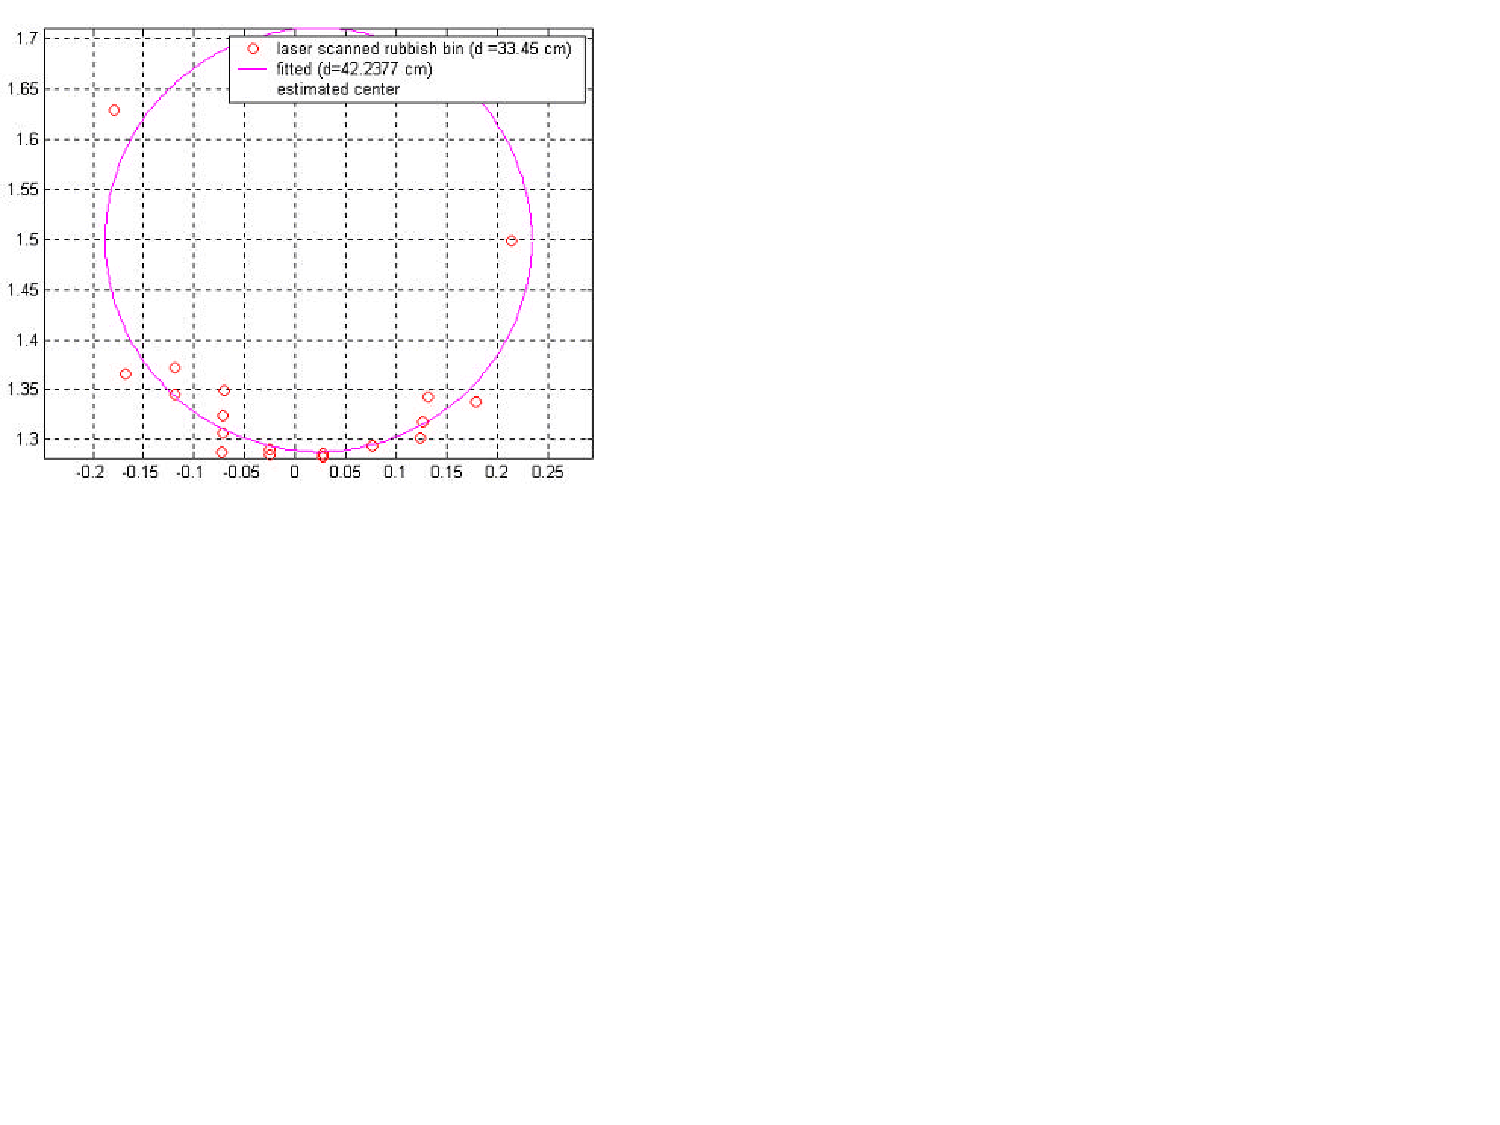
\includegraphics[width=0.45\textwidth]{img/CircleFit} \caption{Circle Fit} \label{fig:CirFit}
\end{figure}








\subsection{Circle Fit with Known Radius}
\label{sec32}


Some of the round objects in the static uncertain environment may have known radii.
So, although simpler, it is practically desirable to perform circle fit with known radius.
Here we use geometrical error for the fit performance index.

%This approach based on algebraic circle fit in order to achieve a better precision. 

Given a set of points with coordination $\{ (x_i,y_i), i=1,2, \cdots, n\} $,   find the best parameters $x_c$ and $y_c$, the center coordinate of the circle
\[
(x-x_c)^2+(y-y_c)^2  - R^2
\]
where $R$ is the known radius, such that the geometric error 
 $\varepsilon = \sum_{i=1}^{n} (\sqrt{ (x_i-x_c)^2+(y_i-y_c)^2 } - R^2)$ 
is to be  minimized.  

Via the gradient of $\varepsilon$ with respect to $x_c$ and $y_c$, an iterative scheme for  $x_c$ and $y_c$ can be formulated and implemented. Since $R$ is known, the convergence process is quite reliable and fast.
%
%$$J=\left[ \matrix{
%\frac{\partial Error}{\partial x_i} & \frac{\partial Error}{\partial y_i} } \right] $$
%$$= \left[ \matrix{
%\frac{(x_i-x_c)}{\sqrt{(x_i-x_c)^2+(y_i-y_c)^2}} & \frac{(y_i-y_c)}{\sqrt{(x_i-x_c)^2+(y_i-y_c)^2}}
%} \right] $$
%Then we can use gradient converge approach to update the origin by
%$$ J h + Error = 0 $$
%$$ \left[ \matrix{x_c & y_c} \right] = \left[ \matrix{x_c & y_c} \right] + h $$




\subsection{Ellipse Fit}
\label{sec33}




The general form of an ellipse is described by
\[
a_1 x^2 + a_2 x y + a_3 y^2 + a_4 x + a_5 y + a_6 =0.
\]
The ellipse fit problem is very similar to the algebraic circle fit method presented in 
Sec.~\ref{sec31}. 

%Given two vector $(\mathbf{x}, \mathbf{y})$ with the same size, solve the equation $ M\mathbf{a} = 0$ by means of least mean square, where 
Here the matrix sent for SVD is given by
$$  \mathbf{D}= \left[\matrix{
x_1^2 & x_1 y_1 & y_1^2 & x_1 & y_1 & 1 \cr
x_2^2 & x_2 y_2 & y_2^2 & x_2 & y_2 & 1 \cr
x_3^2 & x_3 y_3 & y_3^2 & x_3 & y_3 & 1 \cr
\vdots & \vdots & \vdots& \vdots& \vdots& \vdots \cr
x_n^2 & x_n y_n & y_n^2 & x_n & y_n & 1 
} \right] $$
 and $\mathbf{a}= [a_{1},  \cdots,  a_{6}]'$
%
%Same as circle fit, we can do SVD decomposition for matrix $M$, $[U, S, V]= SVD(M)$, and $V=\left[\matrix{%
%v_1 & v_2 & v_3 & \cdots } \right] $. The solution is $v_6$. 


 

\subsection{Plane Fit}
\label{sec3_planefit}



Different from the above fitting method mainly for 1D laser scan data set, the methods of this subsection and the next subsection are designed for 2D laser scanner data processing. Actually, the acquired data from a 2D laser scanner is a 3D  array, as mentioned in Sec.~\ref{sec2}.
The goal of the plane fit problem is to find the optimal coefficients $a_1, a_2, a_3, a_4$, such that
$$   \left[ \matrix{
    x_1 & y_1 & z_1 & 1 \cr
    x_2 & y_2 & z_2 & 1 \cr
    x_3 & y_3 & z_3 & 1 \cr
    \vdots&\vdots&\vdots&\vdots \cr
    x_n & y_n & z_n & 1  }\right]
\times \left[ \matrix{
    a_1 \cr a_2\cr a_3\cr a_4 }\right] =0 $$
has a solution in LS sense. 
Again, here we use the SVD technique for the plane fitting.

%Same as above, SVD is a powerful tool to solve the problem.
%$[U, S, V]=SVD(M)$;
%$v_4$ are the solution of $\left[\matrix{A & B & C & D} \right]^T $.





\subsection{3D Corner Fit/Detection}
\label{sec3_3dcornerfit}

Corner detection is normally studied in the context of 2D image processing. Corner is one of the basic image features and the corner detection has been extensively studied ~\cite{Ruzon99Corner,Smith97Susan}. For 3D corner detection, we can project the 3D corner to a 2D surface and detect the corner in 2D. The advantage of this method is simple. However,    some times it may not be able to detect some corners in certain 3D configurations. Here we propose two effective 3D corner fit algorithms. 

The first method fits an intersection point of 3 planes as the corner. So there is not limitation
on whether the corner is convex or concave. Moreover, the corner is not necessarily to be symmetric. 
The disadvantage of this algorithm  is that it can not fit corner without a prior plane segmentation step. 

This corner fit problem is to find the best corner $\{x^*,y^*,z^*\}$, such that
$$\left[ \matrix{
    A_1 & B_1 & C_1 \cr
    A_2 & B_2 & C_2 \cr
    A_3 & B_3 & C_3 \cr
    \vdots & \vdots& \vdots \cr
    A_n & B_n & C_n } \right]
\times
    \left[\matrix{
    x^* \cr y^* \cr z^* } \right]
+
    \left[\matrix{
    D_1 \cr D_2 \cr D_3 \cr \vdots \cr D_n } \right]
=
    \left[ \matrix{
    e_1 \cr e_2 \cr e_3 } \right]
$$
or $M \times P = -D$, where,  $e_1^2+e_2^2+e_3^2$ is to be minimized the minimum.
Based on the projection theorem, the solution is
$$P =(M^T M)^{-1} M^T (-D)$$
$$\left[\matrix{ x^* & y^* & z^*} \right] = P^T. $$

The second algorithm can fit corners directly from 3D point set. This approach reduces the requirement on segmentation. We can separate points to small subsets, and then fit them by the following corner fit function. The limitation of the algorithm is that the corner function is only suitable for convex and symmetric corners. The proposed corner function is
described by
\[
z=e^{k_1(x-x_0)^2+k_2(y-y_0)^2+k_3}
\]
where $k_1, k_2, k_3, x_0, y_0$ are parameters to be fit. In LS sense, we can re-formulate the above fitting problem into 
    $$\left[\matrix{
    x_1^2 & x_1 & y_1^2 & y_1 & 1 \cr
    x_2^2 & x_2 & y_2^2 & y_2 & 1 \cr
    \vdots& \vdots&\vdots&\vdots&\vdots \cr
    x_n^2 & x_n & y_n^2 & y_n & 1 \cr}\right]
    \left[\matrix{
    c_1 \cr c_2 \cr c_3 \cr c_4 \cr c_5 \cr } \right]
    =
    \left[\matrix{
    \log(z_1) \cr \log(z_2) \cr \vdots \cr \log(z_n) \cr }\right].     $$
And starting from here, it will be the same as in the previous method.

%the $\left[\matrix{c_1 & c_2 & c_3 & c_4 & c_5} \right]$ with minimum norm is the solution we want. This question can be solved by the same approach of the corner fit. 


%\section{Arbitrator}
%If the identity of the object is now clearly known, arbitration is necessary to find the suitable fitting algorithm. $\cdots$.

%{\bf Will be included in the final version}.

%\section{Experimental}
%We did experiments to verify $\cdots$ .

%{\bf Will be included in the final version}




% 

In the final version of this paper,   we will include the section on ``Arbitrator'' or ``Object Decision'' as well as the related experimental results. 



%%%%%%%%%%%%%%%%%%%%%%%%%%%%%%%%%%%%%%%%%%%%%%%%%%%%%%%%%%%%%%%%%%%%%%%%%%%
\section{Concluding Remarks}  
\label{sec6}
%%%%%%%%%%%%%%%%%%%%%%%%%%%%%%%%%%%%%%%%%%%%%%%%%%%%%%%%%%%%%%%%%%%%%%%%%%% 
   
This paper presents some techniques for sensing and perception for an
omnidirectional ground autonomous vehicle equipped with a laser scanner. In an
assumed structured environment (static but uncertain), the sensing data processing methods for both 1D
and 2D laser scanner are discussed. Raw data are segmented to lines, circles,
ellipse, planes and corners by task depended segmentation algorithms.  Each
subset of data is then fit by a known template shape as listed above.  

Our immediate effort is to make use of these medium level information in our  vehicle to infer its relative position with respect to the known landmarks and in turn help to determine its absolute
position on the map, a procedure known as mobile robot localization.
Other future efforts include (1) the motion estimation of dynamic obstacle(s) by assuming that the environment is dynamic uncertain; (2) the fusion with sonar, laser scanner and image sensing information for local map building and
 (3)  relative navigation  without  absolution position information (or inertial/world coordinates) via sensor fusion and spatial filtering.





\section*{Acknowledgment}
The authors would like to acknowledge the fruitful discussions with 
CSOIS members in Vetronics Group and Intelligent Behavior Group. In particular, 
  the authors are grateful to Professor Kevin L. Moore,  Director of CSOIS, for his   support  of this work.
 
\bibliography{csois1,csois2,laser}
 
\end{document}
 

% cut paste this two bib entries in your "laser.bib"

